\ifx\wholebook\relax\else
\input{../Common.tex}
\input{../macroes.tex}
\begin{document}
\fi

\chapter{Composing Methods}\label{ch:composons}

\begin{chapterfigure}
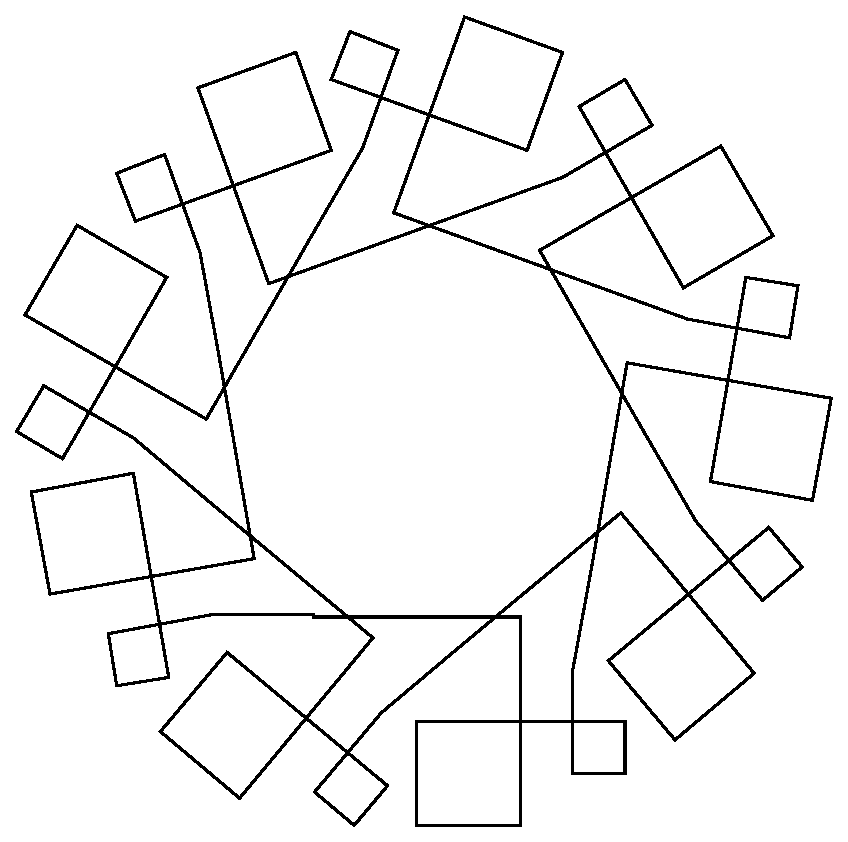
\includegraphics[width=6cm]{compArtNouveauTurningScr}
\end{chapterfigure}

In  Chapter~\ref{ch:turtleTeaching}, you learned how to define methods. We showed that defining methods is interesting because (1) methods avoid to have to rewrite scripts and introduce errors and (2) methods can be used by different robots. The other main advantage of using methods that we are going to explore in this chapter is the possibility to reuse methods, \ie to define a method by calling other methods. Being able to reuse methods is extremely important because we can define a method in terms of another one without having to know all the details of how the second method is defined.  We just call it.

\section{Nothing Really New: the \ct{square} Method}
Composing method is quite natural and it is not really new. Indeed, this is what we made in Chapter~\ref{ch:turtleTeaching} when we defined a method! The method \ct{square} is defined by calling the methods \turnLeft and \timesRepeat. Therefore it is defined in terms of other
methods but we do not have to know how \turnLeft or \timesRepeat are defined. So we are already done with this chapter!

\begin{method}\label{comp:square}
square 
   "Draw a square of 100 pixel size"

   4 timesRepeat: 
         [ self go: 100;
                  turnLeft: 90]
\end{method}


\section{Other Graphical Patterns}
In Chapter~\ref{ch:turtleTeaching}, we asked you to define the method \ct{pattern} that draws a nice pattern (See~\scrref{src:artNouveau}). Now we ask you to follow the experiments and produce the drawings by defining following methods. 

%We remind you the definition of this method if you forgot to save it, so that you can define it now. 
%\begin{methodfig}{compArtNouveauScr}\label{src:mth:artnouveau}
%artNouveau
%   "draws a thing"

%   self go: 100.
%   self turnRight: 90.
%   self go: 100.
%   self turnRight: 90.
%   self go: 50.
%   self turnRight: 90.
%   self go: 50.
%   self turnRight: 90.
%   self go: 100.
%   self turnRight: 90.
%   self go: 25.
%   self turnRight: 90.
%   self go: 25.
%   self turnRight: 90.
%   self go: 50
%\end{methodfig}



\begin{exofigwithsize}[0.5]{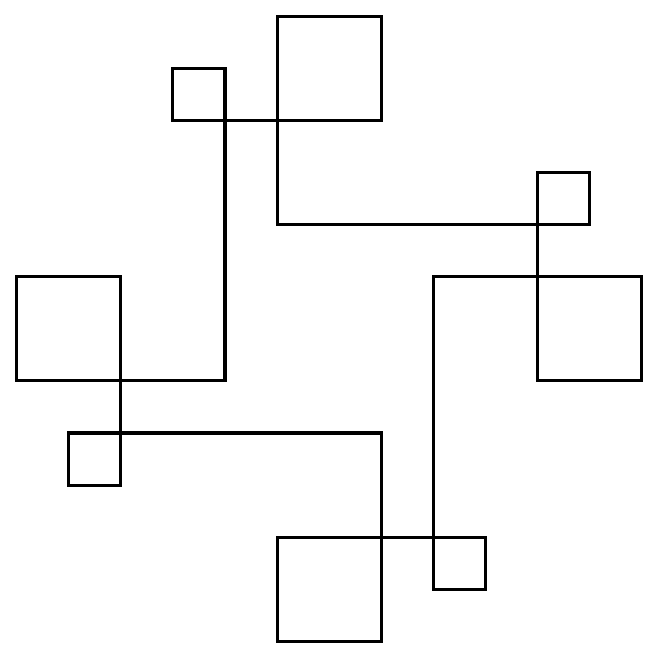
\includegraphics[width=5cm]{compCompleteThing}}
Define the method \ct{pattern4} that calls 4 times \ct{pattern} and produces right figure and that we use  in the script below.

\begin{nalltt}
| \caro |
\caro := \Turtle new.
\caro pattern4
\end{nalltt}
\end{exofigwithsize}

\begin{exonofig}
Define the method \ct{tiltedPattern}  draws the first picture of the Chapter. To help you a bit you have a repeat 9 times the pattern and the angle to turn is 10 degrees.

\end{exonofig}

\hidden{\begin{nalltt}
tiltedPattern 

   9 timesRepeat: 
                  [self pattern. 
                  self turnRight: 10. 
                  self go: 50 ]
\end{nalltt}}


\begin{exofigwithsize}[0.5]{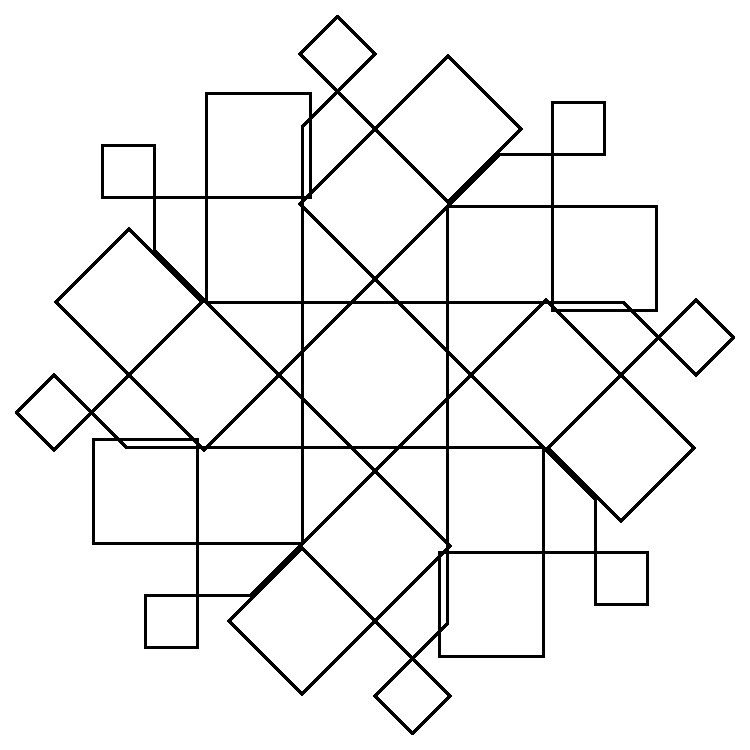
\includegraphics[width=6cm]{compArtNouveauGiantScr}}
Define the method \ct{doubleFrame} that draws the picture on the right. 

\

\begin{nalltt}
doubleFrame

    8 timesRepeat: [self pattern ;
                                     turnLeft: 45 ;
                                     go: 100]
\end{nalltt}
\end{exofigwithsize}


\section{Stepping Back}
Now let us analyze what we learned from the experiments you did. As you can see it with the methods \ct{pattern4}, \ct{tiltedPattern}, and \ct{doubleFrame}, the method \ct{pattern} is only defined once, but reused several times in different methods. Defining \ct{pattern} as a method allows you to: (1) define it only
once, (2) reuse it in various contexts and (3) do not introduce errors during the rewriting of this method. 

If you look at the definition of the method \ct{doubleFrame}, you see that it is defined in terms of \ct{pattern} method that is itself defined in terms of other methods such as \go, \turnLeft...and so on. In fact, a complex method is often defined in terms of simpler methods, which as well are defined in terms of simpler methods too and so on. This is because it is simpler to understand and to define simpler methods.  In Chapter~\ref{ch:recomposing} we shall show you that to solve a problem it is simpler to decompose it in terms of smaller subproblems, solve them and use them to finally solve the first problem. 

It is essential to understand that while defining the method \ct{doubleFrame} we do not to know how \ct{pattern} is defined, we just want to know what is does and to use it!  When we define a method we are giving a name to a sequence of messages and doing so we are reducing the number of details that we have to remember.  We just have to remember what does the method and its name not how it does it.  We say that we are building an \emph{abstraction} over the definition details.

To really show you this point, we rewrote the method
\ct{doubleFrame} without calling the method \ct{pattern}, we directly copied the definition of this method (shown in italic) inside the other one. Compare with the method \ct{doubleFrame} and imagine that we would do the same with the code of \turnRight, \turnLeft, and \go because there are also methods. This would be a nightmare. There would be so much details that we would be lost all the time. 

\begin{method}
doubleFrameWithoutCallingArtNouveau

   8 timesRepeat: [\textit{self go: 100.
                  self turnRight: 90.
                  self go: 100.
                  self turnRight: 90.
                  self go: 50.
                  self turnRight: 90.
                  self go: 50.
                  self turnRight: 90.
                  self go: 100.
                  self turnRight: 90.
                  self go: 25.
                  self turnRight: 90.
                  self go: 25.
                  self turnRight: 90.
                  self go: 50thing.}
                  self turnLeft: 45. 
                  self go: 100]
\end{method}



\largecadre{We define a method in terms of other ones and this at various levels
without having to know how these methods themselves are defined.}

\section{Squares Everywhere}
Now it is time for you to practice. Define the following methods using the method \ct{square}.


\begin{exonofig}{Some Boxes.}
Define the methods \ct{box} and \ct{separatedBox} that produce the 
pictures shown in Figure~\ref{c7groscarre}.
\end{exonofig}

\begin{figure}[!htbp]
\begin{minipage}[c]{.4\linewidth}
\centerline{\includegraphics[width=\linewidth]{comp4Squares}}
\end{minipage}
\hfill
\begin{minipage}[c]{.4\linewidth}
\centerline{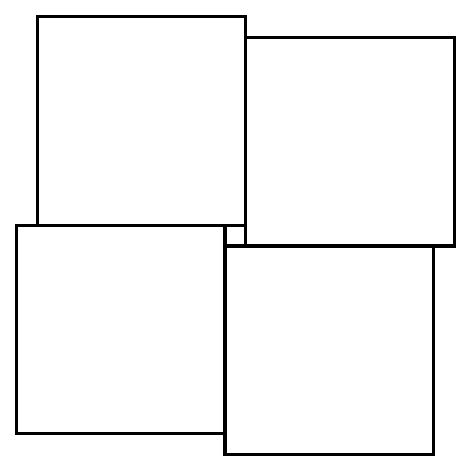
\includegraphics[width=\linewidth]{comp4SquaresTwo}}
\end{minipage}
\label{c7groscarre}
\end{figure}
 

\hidden{
| caro |
caro := Turtle new.
4 timesRepeat: [caro square100.
               caro turnLeft: 90]

| caro |
	caro := Turtle new.
	4 timesRepeat: 
		[ caro compSquareL100.
        caro turnLeft: 90. 
		caro go: 10]
}

\begin{exonofig}
Modifying your previous methods to generate various figures.
\end{exonofig}

\hidden{
\begin{alltt}
| caro |
caro := Turtle new.
12 timesRepeat: [caro square100.
                caro turnLeft: 30.
                caro go: 10]
\end{alltt}}

\begin{exonofig}{Star.} 
Using the method \ct{box}, experiment and define a method \ct{star} that produce the right picture in Figure~\ref{c7star}
\end{exonofig}

\begin{figure}[!htbp]
\begin{minipage}[c]{.4\linewidth}
\centerline{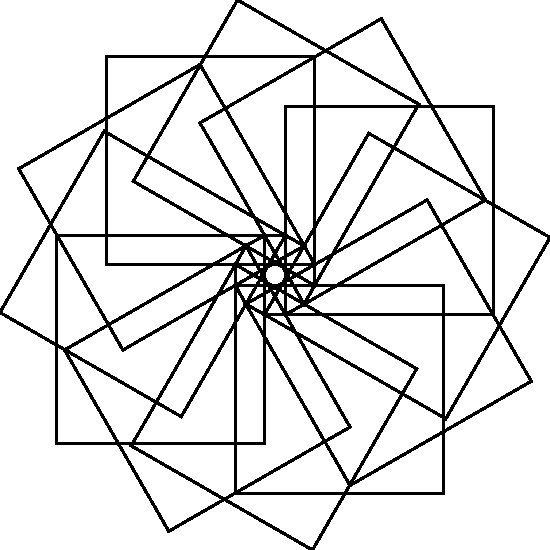
\includegraphics[width=5cm]{comp4SquaresThree}}
\end{minipage}
\hfill
\begin{minipage}[c]{.4\linewidth}
\centerline{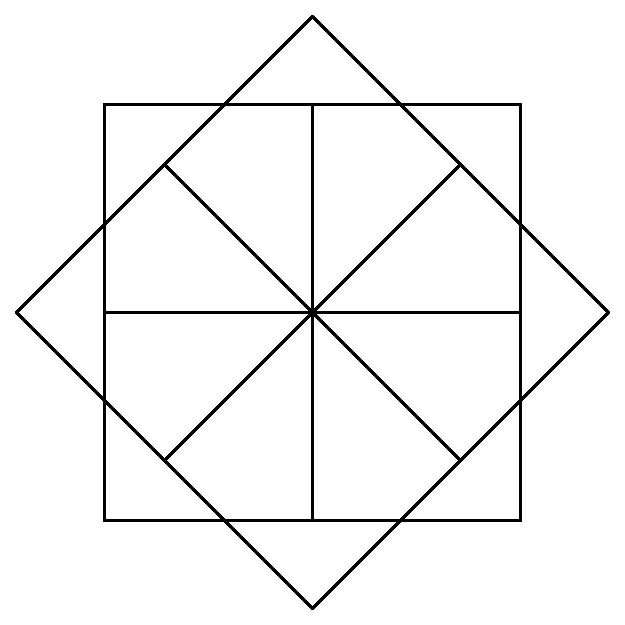
\includegraphics[width=5cm]{comp4SquaresFour}}
\end{minipage}
\label{c7star}
\caption{Stars}
\end{figure}


\summa

We can define a method in terms of other ones and this at various levels without having to know how these methods themselves are defined.


\ifx\wholebook\relax\else
\end{document}\fi
